\subsection{Formal BON}
\subsubsection{Variance}
\label{implementation-variance}
\begin{figure}[H]
{\footnotesize
\begin{verbatim}
 1| conforms_to (other): BOOLEAN
 2|  do
 3|    Result := name of Current is equal to ANY
 4|    if not Result and name of other is not NONE then
 5|       if name of Current is equal to name of other then
 6|          if Current.generic_count = other.generic_count then
 7|              if Current.has_actual_type and other.has_actual_type
 8|                 Result := Current.instance_equality (other)
 9|              elseif Current.has_actual_type xor other.has_actual_type then
10|                 Result := False
11|               else
12|                  Result := Current.generics = other.generics
13|               e nd
14|           end
15|        else
16|         Result := exists an ancestor a' of Current such that a'.conforms_to(other)
17|        end
18|    end
19|  end
\end{verbatim}
}
\caption{Example of a generic class specification with type bounds}
\label{fig:generic_class_specification_bounded}
\end{figure}

\textit{conforms\textunderscore to}

\subsubsection{Features}
At the heart of a class specification are its features, the relations of which are discussed in this section. Features are represented in the type checker by the class \textsc{tbon\textunderscore tc\textunderscore feature}. As mentioned in section \ref{implementation-context-class-structure}, a class in the type context is associated with a set of instances of these. In turn, a feature is associated with its arguments through a list of instances of \textsc{tbon\textunderscore tc\textunderscore feature\textunderscore argument}. 
\subsubsubsection{Feature Status}
Whenever a feature exists in a class specification in which ancestors are specified, it can potentially have a precursor. Luckily, because features repeatedly effect, undefine, and redefine each other all the way down the inheritance hierarchy, only the nearest precursor feature needs to be considered when determining whether a feature specification is well-typed. The status of a feature is implemented by simple boolean flags in \textsc{tbon\textunderscore tc\textunderscore feature}; and as specified in the grammar in \cite{walden1995}, only one (or none) of these can be set at any given time.
\begin{figure}[H]
    \centerline{\scalebox{0.75}{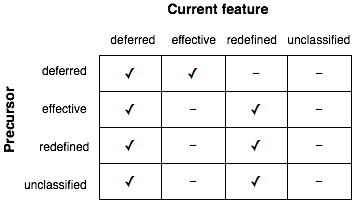
\includegraphics{images/feature_status.png}}}
    \caption[Feature status matrix]{Allowed status relations between a feature and its precursor}
    \label{fig:feature_status}
\end{figure}
Figure \ref{fig:feature_status} shows the allowed relations between the status of the precursor and the status of the current feature (i.e. the feature whose well-typedness is being determined). Notably, what it shows is that it is always possible to undefine an inherited feature by creating a \textit{deferred} version of it in the current class, regardless of the status of the precursor. This becomes relevant in any situation in which one wants to ensure that all concrete descendants of the current class redefines (or, more precisely, effects) the undefined feature.

As for the \textit{effective} status, the restrictions for it may seem overly constraining at first, when considering that the original specification of it states that "[the effective marker] may also be used just to emphasize that the feature will have an implementation," \cite[p.~40]{walden1995}. However, figure \ref{fig:feature_status} only status that \emph{if} a precursor exists for an \textit{effective} feature, then it must be \textit{deferred}; if no precursor exists, one may use it freely.

The \textit{redefined} status is defined as one would expect from the definition in \cite[p.~40]{walden1995}. The only noteworthy aspect is that if a precursor is \textit{deferred}, the current feature must be marked as \textit{effective}, as conceptually, one cannot redefine something that has yet to be defined.

For unclassified features, the definition is straightforward: an unclassified feature defined in the current class can never have a precursor. An unclassified feature inherited from an ancestor can be redefined and undefined as expected, though.
\subsubsubsection{Prefix and Infix Features}
For regular features, having two features with identical names in the same class (either directly defined in the class or inherited) is not allowed; this is not true for prefix and infix features. For instance, it should be possible to define the operator ''+'' as both a unary and a binary operator on an object, e.g. an integer. The really interesting aspects of prefix and infix features arises when they are used, though, which will be described in the formal assertions section.

\subsubsection{Generics}
\label{implementation-generics}
In textual \textsc{bon}, formal specifications can involve generics in several different ways:
\begin{itemize}
\item Class specifications, e.g. \textsc{list}[\textsc{e}]
\item References to formal generic names of enclosing class,\newline e.g. \textit{first\textunderscore element}: \textsc{e}
\item Generic class specifications instantiated with concrete types,\newline e.g. \textit{string\textunderscore list}: \textsc{list}[\textsc{string}]
\item Generic class specifications instantiated with formal generic names of enclosing class, e.g.  \textit{element\textunderscore list}: \textsc{list}[\textsc{e}]
\end{itemize}
Note that the first and the last example both refer to \textsc{list}[\textsc{e}], but in very different respects: the former is a specification of a new class \textsc{list} with one (unbounded) type parameter \textsc{e}, while the latter is an instantiation of the same class, in which it is assumed that the enclosing class of the feature \textit{element\textunderscore list} has a (possibly bounded) type parameter \textsc{e}. How each of these types of generics are handled by the type checker is explored in this section.
\subsubsubsection{Generics in Class Specifications}
%Generics - explain association between bounding type and actual type.
As mentioned in section \ref{implementation-context-class-structure}, classes in the context are associated with type parameters through a sequence of instances of \textsc{tbon}\textunderscore \textsc{tc}\textunderscore \textsc{generic}. The class \textsc{tbon}\textunderscore \textsc{tc}\textunderscore \textsc{generic} has two notable attributes: \textit{bounding\textunderscore type} and \textit{actual\textunderscore type}. The attribute \textit{bounding\textunderscore type} represents the type bound of the formal generic name of the type parameter. Accordingly, the \textit{actual\textunderscore type} represents the concrete type associated with the formal generic name.

\begin{figure}[H]
{\footnotesize
\begin{verbatim}
1| static_diagram
2| component
3|       class NUMBER_LIST [E -> REAL]
4| end
\end{verbatim}
}
\caption{Example of a generic class specification with type bounds}
\label{fig:generic_class_specification_bounded}
\end{figure}

In the type context, no generic class specifications have any actual types associated with any of its type parameters; these are only present in instances of these, which will be discussed next. To exemplify, consider the case presented in figure \ref{fig:generic_class_specification_bounded}. Here, the class \textsc{number\textunderscore list} would exist in the type context, and have a single type parameter with a formal generic name \textsc{e} and a \textit{bounding\textunderscore type} attribute pointing to the type \textsc{real} (which would also exist in the type context in order for the specification to be well-typed). The \textit{actual\textunderscore type} attribute of the type parameter would point to \textit{Void}, as this example is not an instantiation of the type in question, but a specification.

As a result of this, and to differentiate between them, there is no equivalence relation between a class specification (without any actual types) and an instance of this class (with actual types), as they in practice are two different types. They are not unrelated, however, as will be explained next.
\subsubsubsection{Instantiation of Generic Types}
Because a generic class specification only specifies a family of concrete classes that have a common base type,  it has to be instantiated with concrete types to be of any practical use.  One could say that a generic class specification merely acts as a template for such concrete instances (in some languages, such as C++, generic classes are explicitly denoted \textit{templates} \cite{stroustrup1997}), and therefore it is not possible to refer directly to a generic class specification in places where a concrete type is expected; in textual \textsc{bon}, these places include feature types, feature argument types, formal assertions, and interestingly, type bounds in generic class specifications. In order to instantiate a generic type, a mechanism that ambiguates between the generic class specification and an instantiation of it is needed, while still ensuring that the instantiated type has all the same attributes (e.g. features) of the generic class specification.
\paragraph{} All types eligible for participation in the instantiation of a generic type are found in the type context after the first phase. Whenever an instantiation of such a type occurs, for instance as a feature type, the type checker [...]:
\begin{enumerate}
\item Creates a deep copy of the generic class
\item Registers the copy in the generic class as an instance of that class
\item Adds the concrete type parameters as actual types to the generics of the copied class
\end{enumerate}
In practice, the first two steps happen as a single call to the \textit{new\textunderscore instance} feature of the generic class, the specification of which is found in the type context. As such, the individual instantiations of a generic class are not added directly to the type context. Instead, each generic class keeps track of all the instantiations that have been made of it. The benefit of this approach is that whenever the generic class is updated, i.e. an ancestor or a feature is added in the second phase, the generic class can update all of the instantiations of it accordingly. Consequently, when an instance is registered as an instance (step 2 in the above enumeration), one can think of it as an observer observing the generic class, which then notifies/updates the instantiations whenever a change occurs.
\paragraph{} In step 1 above, it is noted that a \emph{deep} copy is created. This is an important aspect because, as previously explained, type parameters of a class are implemented by associating a type with a sequence of instances of \textsc{tbon}\textunderscore \textsc{tc}\textunderscore \textsc{generic}. If only a shallow copy was created, the copy would refer to the exact same type parameters as the original, thus making it impossible to add individual concrete actual types to each of these parameters for each instance without affecting the original generic specification.
\subsubsubsection{References to Generic Types}
The instantiation of generic classes explained above happens every time a reference to a concrete type is expected and a generic type is provided in the abstract syntax.
\begin{figure}[H]
{\footnotesize
\begin{verbatim}
1| static_diagram
2| component
3|       class MAP [K -> INTEGER, V]
4|       class MAP_CLIENT
5|          feature
6|             string_map: MAP [INTEGER, STRING]
7|          end
8| end
\end{verbatim}
}
\caption{Example of a reference to a generic type}
\label{fig:ref_generic_type}
\end{figure}
In the example in figure \ref{fig:ref_generic_type}, an instantiation of the generic type \textsc{map} is shown. At the time the type checker resolves the feature \textit{string\textunderscore map} (at the end of the first phase), the generic class specification (with no actual types, although the first type parameter has a type bound of type \textsc{integer}) of the type \textsc{map} exists in the type context. To resolve the feature, the resolving code recognizes that \textsc{map} has type parameters, and therefore creates a new instance of \textsc{map} to which the feature can refer (steps 1 and 2 in the previous section). Furthermore, the concrete type \textsc{integer} is added as actual type to the first parameter of the new instance, and \textsc{string} is added as actual type to the second parameter. As such, the feature  \textit{string\textunderscore map} now refers to a separate instance of \textsc{map}, which has all the features of the generic class from which it originates plus the added actual types.
%Covariant conformance between bounds
\paragraph{} In order for this new instance to be well-typed, the type of the first concrete parameter type must conform covariantly to the bounding type of the first parameter of the class specification, \textsc{k} (just as defined for feature types and feature argument types in section \ref{design-type-system}). Textual \textsc{bon} has no construct for differentiating between different types of variance for type parameters, which is known from languages such as Java and C\#, and enforcing covariant conformance is thus a design decision on the part of the type checker. This decision mainly based upon the fact that the Eiffel language also enforces covariant conformance of type parameters \cite[Constrained~genericity]{meyer2001}. Future versions could include a switch to fine-tune this aspect of type checking.

As described in section \ref{implementation-variance}, this conformance check also happens through the feature \textit{conforms\textunderscore to}. In the presented example, the concrete type trivially conforms to the bounding type, as they are both \textsc{integer}. Some non-trivial situations, however, require a little more consideration.
\subsubsubsection{Solutions to Non-trivial Generics Situations}
The first non-trivial situation considered is presented in figure \ref{fig:non_conforming_type_bounds}.
\begin{figure}[H]
{\footnotesize
\begin{verbatim}
1| static_diagram
2| component
3|    class SEQUENCE [G -> REAL]
4|    class CLIENT_CLASS [H]
5|       feature
6|          seq: SEQUENCE [H]
7|       end
8| end
\end{verbatim}
}
\caption{Situation 1) Example of non-conforming type parameter bounds}
\label{fig:non_conforming_type_bounds}
\end{figure}
In this example, the feature \textit{seq} instantiates the class \textsc{sequence} with the type parameter \textsc{h} of the enclosing class \textsc{client\textunderscore class}. The type parameter of \textsc{sequence} is bounded by \textsc{real}, while the parameter \textsc{h} has no bound; so how can it be determined if \textsc{h} is a legal parameter, which makes the instantiation well-typed? Intuitively, one might say that if the type parameter has no bounding type, nothing at all can be said about it -- it could be anything. And by following that intuition, the answer is given: if \textsc{h} has no explicit bounding type, it is implicitly bounded by \textsc{any}, which is the base class of all classes. This mimics the behaviour found in Eiffel, in which unconstrained type parameters are also considered to be bounded by \textsc{any} \cite[p.~77]{meyer2001}.

Now, is the example then well-typed? No, because the concrete type parameter of an instantiation must conform to the bounding type of the type parameter in the class specification, and the only thing known about \textsc{h} is that it has type \textsc{any}, the example is not well-typed, as \textsc{any} does not conform to \textsc{real}.
\paragraph{} The second situation contain similar, but different, subtleties.
\begin{figure}[H]
{\footnotesize
\begin{verbatim}
1| static_diagram
2| component
3|    class SEQUENCE[G]
4|    class A [E -> SEQUENCE[REAL]]
5|    class B [M -> SEQUENCE[INTEGER], N -> A[M]] 
6| end
\end{verbatim}
}
\caption{Situation 2) Specification of a generic class with generic type bounds}
\label{fig:generic_type_bounds}
\end{figure}
Firstly, the differences between the three instantiations of the class \textsc{sequence} should be noted (also note that in this example, the type parameter of \textsc{sequence} has no bounding type). Secondly, the example shows a type parameter \textsc{n} that is bounded by a generic class \textsc{a} instantiated with the first parameter of class \textsc{b},  \textsc{m}. Instantiating a bounding type with another type parameter is permitted, as long the type parameter used in the instantiation is declared at the time of its use (i.e. the type parameter appears to the left of the type parameter that uses it in its specification).

What happens in this case is that \textsc{m} is considered to be a sequence of \textsc{integer}, while the type parameter of \textsc{a} is bounded by a sequence of {real}. At the time of the instantiation of class \textsc{a} for the bound of type parameter \textsc{n}, the bounding type of \textsc{m} has to conform to the bounding type of \textsc{a} in order for the instantiation to be well-typed. But, as already defined in section \ref{design-type-system}, the type checker does not consider a sequence of \textsc{real} to conform to a sequence of \textsc{integer}, even though \textsc{integer} might be a subtype of \textsc{real}. Consequently, to make this situation well-typed, one would have to change the bounding type of either type parameter \textsc{e} or \textsc{m}, such that they become equal.

\subsubsection{Formal Assertions}
\label{implementation-formal-assertions}
\label{implementation-def-boolean-type}
\label{implementation-set-expressions}